\section{Инфологическое проектирование}

\subsection{Цель автоматизации предметной области}

Цель автоматизации предметной области --- удовлетворение потребностей клиентов и сотрудников железнодорожных касс в получении и обработке информации о железнодорожных билетах.\par 

\vspace{0.8cm}

\subsection{Основные процессы в предметной области}

Опишем основные процессы в предметной области:
\begin{itemize}
\item получение информации о билетах;
\item получение информации о маршруте следования;
\item учёт проданных билетов;
\item хранение информации о рейсах и направлениях.
\end{itemize}

Составим <<черный ящик>> для описанных процессов и декомпозируем его:

\begin{figure}[h!]
    \centering
    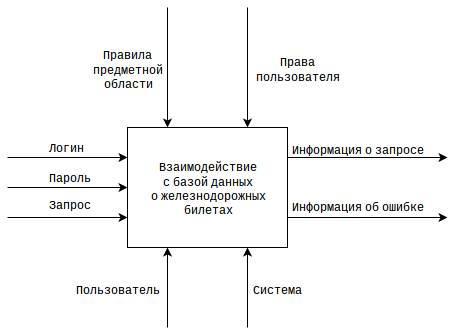
\includegraphics[width=0.7\textwidth]{1}
    \caption{Черный ящик}
    \label{img:1}
\end{figure}

\clearpage

\begin{figure}[h!]
    \centering
    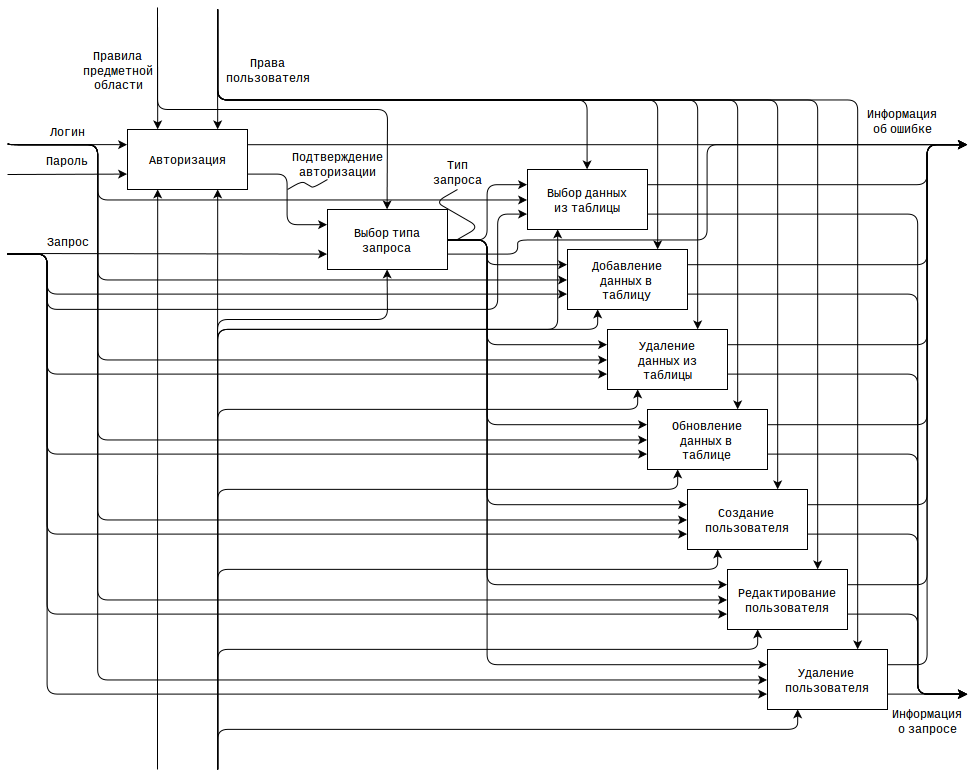
\includegraphics[width=1\textwidth]{2}
    \caption{Декомпозиция <<черного ящика>>}
    \label{img:2}
\end{figure}

\subsection{Основные объекты, сущности и их атрибуты, первичные и внешние ключи}

Опишем основные компоненты (сущности) выбранной предметной области:

    \begin{itemize}
        \item маршрут, атрибуты: станция отправления, станция прибытия, номер маршрута;
        \item рейс, атрибуты: маршрут, дата-время отправления, дата-время прибытия;
        \item вагон, атрибуты: рейс, номер, тип вагона, количество мест;
        \item место, атрибуты: вагон, номер, тип места, цена, занятость;
    \end{itemize}

\vspace{0.8cm}

\subsection{Концептуальная модель базы данных}

Используя сущности, описанные в пункте 3.3, построим концептуальную модель базы данных и обозначим в ней связи между сущностями: 

    \begin{itemize}
        \item маршрут - рейс: один ко многим;
        \item рейс - вагон: один ко многим;
        \item вагон - место: один ко многим.
    \end{itemize}

\vspace{0.8cm}

\subsection{Основные бизнес-правила предметной области}

Определим основные бизнес-правила выбранной предметной области:

    \begin{itemize}
        \item цена билета может зависеть не только от типа вагона, но и от расположения самого места;
        \item продажа билетов осуществляется только на весь маршрут целиком, от начальной станции, до конечной станции;
        \item в маршруте следования учитываются только начальная станция и конечная станция;
        \item количество вагонов в поезде зависит от даты и времени отправления и прибытия;
        \item вагоны нумеруются последовательно, от начала состава;
        \item места нумеруются последовательно, от начала вагона;
        \item дата и время отправления и прибытия указываются по всемирному координированному времени (UTC).
    \end{itemize}
\clearpage